\documentclass[letterpaper]{article}
\usepackage{aaai}
\usepackage{times}
\usepackage{helvet}
\usepackage{courier}
\usepackage{graphicx}
\usepackage{amssymb}
\frenchspacing
\pdfinfo{
/Title (Hashing for Lightweight Episodic Recall)
/Subject (AAAI Publications)
/Author (Scott A. Wallace, Evan Dickinson, Andrew Nuxoll)
/Keywords(Episodic Memory,Soar,Reinforcement Learning,Hidden State)
}
\setcounter{secnumdepth}{0}

\begin{document}
\title{Sudoku Solver}
\author{
	Benjamin Longbons\and
    Eric Klinginsmith \and
    Sebastian S\'{a}nchez \\
Washington State University Vancouver \\
14204 NE Salmon Creek Ave. \\
Vancouver, WA 98686
}

\maketitle
\begin{abstract}
This document explores the performance of two separate implementations of Sudoku puzzle agent and the resulting evaluation of the implementations. Each implementation is a distinct search method to solve any Sudoku puzzle. They will be evaluated based on how fast each solves a given set of puzzles. It was our goal to explore these methods to ultimately see how well they worked.
\end{abstract}

\section{Introduction}

A Sudoku puzzle like the one in Figure \ref{fig:sudoku-puzzle} is any $ n^{2} $ by $ n^{2} $ grid subdivided into $ n^{2} $, n by n squares. In the typical case $ n $ is equal to $3$ which makes the Puzzle a $9$ by $9$ grid with $9$ squares, each square being it's own $3$ by $3$ grid. In any case, to solve the Puzzle, distinct numbers $1$ through $ n^{2} $ must be filled into every row and column of the grid, so that no two numbers are in the same row, column, or square. Our implementations solve any Sudoku puzzle with an $n \le 7$. All of our approaches use partial state.

\begin{figure}[h]
	\centering
	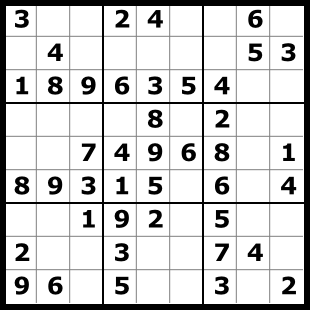
\includegraphics[width=60mm]{./Sudoku-games.png}
	\caption{Sudoku Puzzle}
	\label{fig:sudoku-puzzle}
\end{figure}

\section{Terminology}

\begin{itemize}
\item \emph{Order}: The most basic measure of a puzzle's size, labeled $n$.
\item \emph{Grid}: A square 2-dimensional array of Cells. Both dimensions of the array are $ n^2 $.
\item \emph{Cell}: A single place that can store a number. In a partial state, it may also be blank.
\item \emph{Row}: A horizontal slice of a Grid. It must contain all the numbers $ 1 $ to $ n^2 $ exactly once.
\item \emph{Column}: A vertical slice of a Grid. It must contain all the numbers $ 1 $ to $ n^2 $ exactly once.
\item \emph{Square}: An aligned $ n \times n $ slice of a Grid. It must contain all the numbers $ 1 $ to $ n^2 $ exactly once.
\item \emph{Neighbor} of a Grid: a Grid that differs by adding a value to a single Cell that previously had no values. The core function in all solvers is to iterate over all the Neighbors of a Grid at a certain Cell. For convenience, the Neighbors of a Grid at a Cell that already has a value is sometimes defined as the same Grid.
\end{itemize}

\section{Implementations}

\subsection{Stupid Monkey Brains}

\subsubsection{Stupid}
The Stupid Implementation was chosen as a baseline, and simply iterates over every cell, and recursively checks all Neighbors at that Cell. It performs terribly when the first Cells visited are relatively unconstrained and it guesses wrong, but this Implementation \emph{was} useful to demonstrate the completeness of the general recursive approach.

\subsubsection{Monkey}
The Monkey Implementation was a deliberately naive attempt to improve on the efficiency of the Monkey, particularly for the worst cases, by statically ordering the Cells according to their initial neighbor count. Surprisingly, it actually performed worse in the few tests given to it, though as both implementations are very slow, it cannot be ruled out that the difference is just noise. This implementation also changed the algorithm slightly to skip over already filled cells.

\subsubsection{Brains}
The Brains Implementation was a serious attempt to continue doing the best thing as the puzzle iteratively got closer to solved. It works by calculating, at each step, the number of neighbors at each yet-unfilled cell, and choosing the one with the least number of possibilities. Using this, it achieves pretty good performance for most puzzles. However, there is still a lot of variation, so it is not yet fully optimized.

\subsubsection{Possible Improvements}
The Brains approach still suffers from two major flaws:
\begin{itemize}
\item It recalculates the list of best nodes every step. It would be better to remember a list of most-constrained Cells and update it.
\item It always calculates possible neighbors from $ 1 $ to $ 9 $. This will behave badly if larger numbers are more constrained.
\end{itemize}
Combined, these indicate the reason that certain puzzles take much more time to solve with this solver compared to the next.

\subsection{SearchNxN Implementation}
The SearchNxN Implementation searches for the solution by filling in one square at a time. To do this, SearchNxN first selects one of the squares to fill in. Once selected, SearchNxN will generate all possible solutions for the given square. These these solutions are added to a stack. Then for every element on the stack SearchNxN selects the next square to fill in. This process is repeated until either all squares are filled in, or the stack is empty. If all squares are filled in, then the solution is printed to stdout. Otherwise, there is no solution and \emph{false} is returned. The inspiration behind this method was taken from the common computer science problem of a three coloring. A three coloring is a problem in which when given a map with $n$ regions to color an agent finds a way to color the entire map with only three colors so that no two regions have the same two colors. If we think of the Sudoku puzzle as being a map where no two numbers can be in the same row, column, or square and each square is a region, then a so called three coloring of a Sudoku puzzle would be to "color" each square so that there are no violations where a color would be one of the possible solutions to that square.

\subsubsection{About choosing a the next square}
We would like to now talk about how SearchNxN selects the next square to fill in. There where two types of selection methods within this implementation. These are:
\begin{enumerate}
\item inOrder
\item mostAdjacent
\end{enumerate}

\subsubsection{inOrder}
inOrder is the simplest implementation of the two. I simply fills in each square one at a time left to right top to bottom. Although this method is simple, the time complexity to get the next square is constant.

\subsection{mostAdjacent}
mostAdjacent is a little more complicated. It chooses the square that has the most unfilled squares in the same row or column as that square. For example, Figure \ref{fig:num-sudoku-puzzle} if we assume square $1$, $2$, and $8$ are filled in, then square $1$ has $3$ unfilled in squares in the same row and column has it, square $4$ has $4$ unfilled in squares, square $5$ would have $2$, and so on and so forth. This method was developed to try an eliminate the branching factor of future squares. The idea was the square with the most unfilled squares on the same row and column of it would limit the most possibilities for future squares. This supposedly would make SearchNxN faster than the inOrder method. To find out if this was true we ran some early tests and found that this was not true at all. It turns out that mostAdjacent took $30$ mins to solve v.s. inOrder which only took $2$ mins. This led us to scrap the mostAdjacent method and go with inOrder.

\begin{figure}[h]
	\centering
	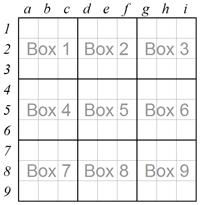
\includegraphics[width=60mm]{./numBox.png}
	\caption{Numbered Sudoku Puzzle}
	\label{fig:num-sudoku-puzzle}
\end{figure}

\subsubsection{About sole candidates}
We would like to mention one other part to our implementation. This is the idea of sole candidates. In a Sudoku puzzle, there are sometimes cells where only one number can be placed there. This means that any partially solved puzzle can have one or more sole candidates. If a sole candidate is found, then our implementation will try to find another. This continues until either all the sole candidates have been found, or it hits a cell where there are no possibilities. If the result is the latter, then that branch of the search is invalid and therefore the search must then try a different path to find the solution. If there are no other branches to explore and a solution has not been found then there is no solution to the given puzzle.

\subsubsection{Possible improvements}
There are several things that could be done to improve the SearchNxN implementation. These are:
\begin{enumerate}
\item Find a way to select a the next square to fill in that is faster than the inOrder method.
\item Implement an arc consistency check beyond the sole candidates.
\item Work on getting parts of the existing code to be more efficient by making critical functions less redundant. 
\end{enumerate}
The above ideas are all things that could make our implementation go from okay to great.

\section{Experiments}
Benchmarks were performed on only two strategies due to computational resource constraints. The strategies used to collect data were SearchNxN and Brains. The data collected was the time each strategy took to solve a Sudoku puzzle. The timer started before the search function in each strategy, and it stopped after the puzzle was solved. About $1300$ $3 \times 3$ Sudoku puzzles were solved using the strategies mentioned above and, outliers were eliminated from the data by taking the top 90\% of the data set sorted from lowest to highest, and were run using a computer with the following specifications.\\

Intel(R) Core(TM) i7-2635QM CPU @ 2.00GHz\\
\indent Memory Ram 8 GBs\\
\indent Linux version 2.6.32-279.19.1.el6.x86\_64

\subsection{SearchNxN Performance}
Now lets look at the performance of the SearchNxN implementation.There are several different ways we measured the performance of the SearchNxN implementation. The way we choose to look at it was the more puzzles that solved within a certain amount of time the better. Figure \ref{fig:search-time-complex-hist} shows what percentage of puzzles this method solved per time 5 second time intervale.

\begin{figure}[h]
	\centering
	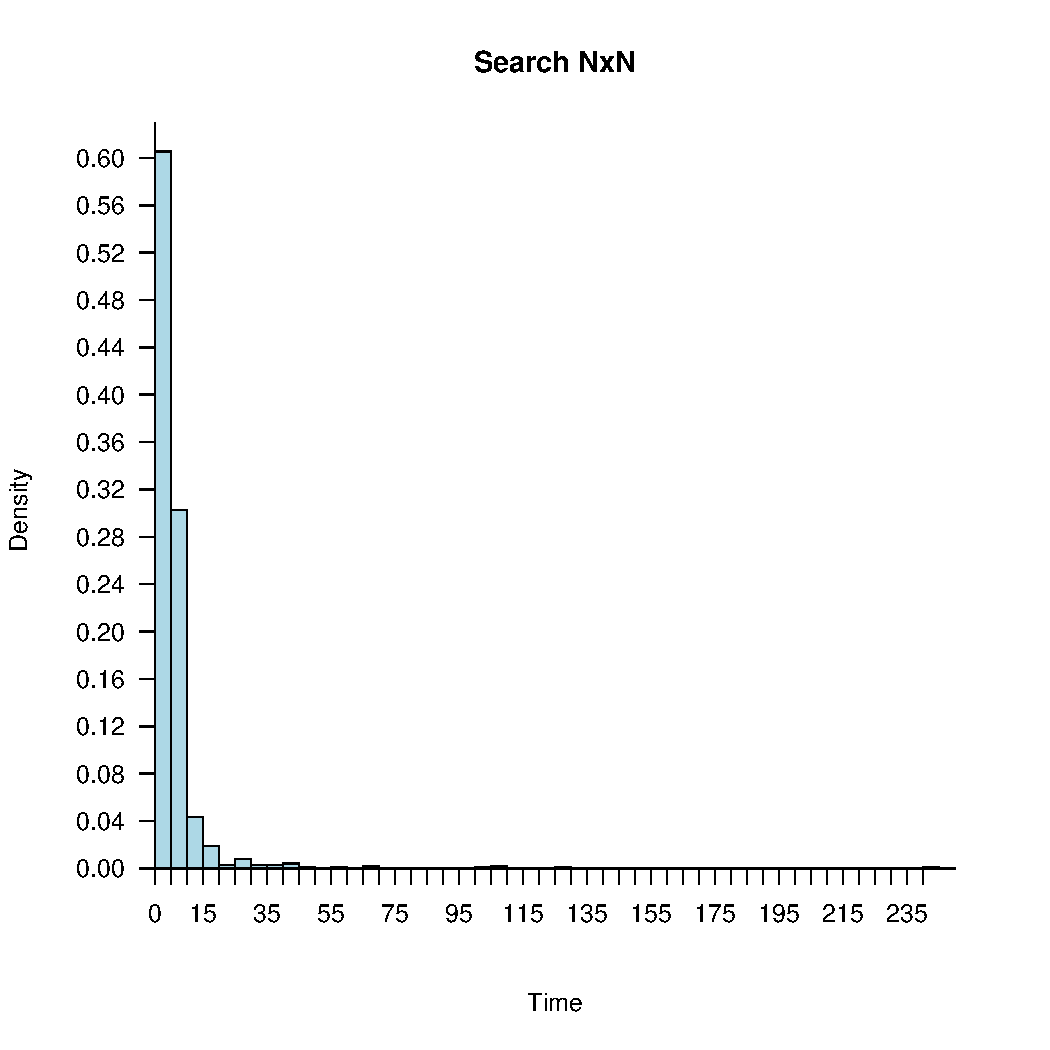
\includegraphics[width=100mm]{../stats/searchNxNEasy.pdf}
	\caption{Histogram of SearchNxN method}
	\label{fig:search-time-complex-hist}
\end{figure}

This shows that about $62\%$ of the puzzles were solved within $5$ seconds, and about $30\%$ of the puzzles were solved from $5$ to $10$ seconds. This graph also includes the outliers, which are on the far right of the graph. The most extreme outlier holds a time of around $240$ seconds and takes up less than $1\%$ of the total puzzles.

In addition this data was tabulated to show statically our results if Table \ref{tab: SearchNxNTab1}.

\begin{table}[h]
\begin{tabular}{|l|l|l|l|l|l|}
\hline
Min. & 1st Qu.  & Median & Mean & 3rd Qu. & Max.\\
\hline
1.000 & 2.272 & 3.909 & 6.211 & 7.016 & 240.700\\
\hline
\end{tabular}
\caption{Statistical data for SearchNxN}
\label{tab: SearchNxNTab1}
\end{table}

However, looking at the data with the outliers is not quite representing the normal case. Therefore, we also made a histogram for the top $90\%$ of the data. This resulted in Figure \ref{fig:search-time-complex-hist-90}.

\begin{figure}[h]
	\centering
	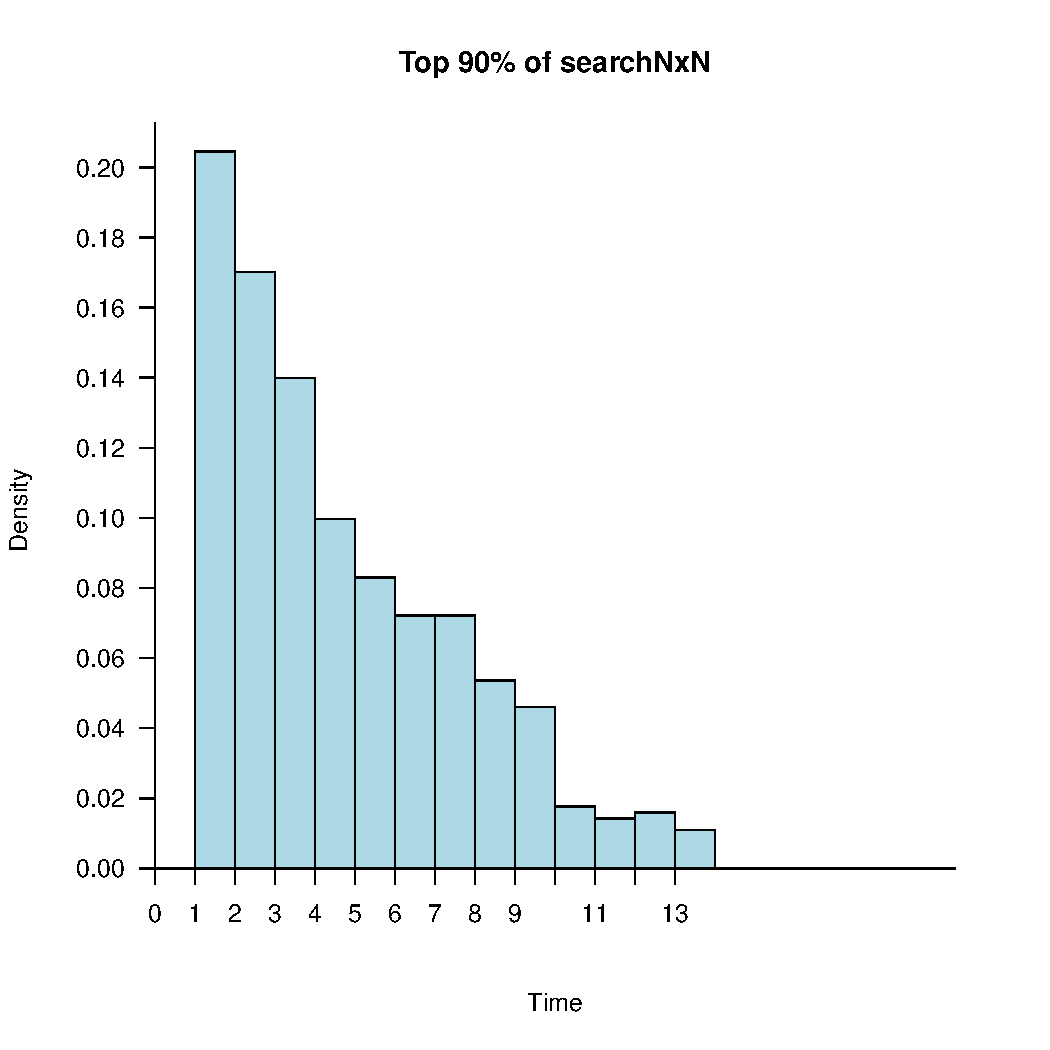
\includegraphics[width=100mm]{../stats/Top90SearchNxN.pdf}
	\caption{Histogram of SearchNxN method of the top 90\%}
	\label{fig:search-time-complex-hist-90}
\end{figure}

As one can see about $20\%$ of these puzzles were solved between $1$ and $2$ seconds and there are no puzzles that took longer than $14$ seconds. This data shows that when we ignore the outliers, most of the puzzles solve in a reasonable amount of time. In addition statistical data has been provided in Table \ref{tab:SearchNxNTab2}.

\begin{table}[h]
\begin{tabular}{|l|l|l|l|l|l|}
\hline
Min. & 1st Qu.  & Median & Mean & 3rd Qu. & Max.\\
\hline
1.000 & 2.298 & 3.870 & 4.705 & 6.747 & 13.830\\
\hline
\end{tabular}
\caption{Statistical data of SearchNxN top 90\%}
\label{tab:SearchNxNTab2}
\end{table}

As one can see the data sports the Histogram by showing that the mean is right around $5$ seconds and the Max is right around $14$.

\subsection{Brains Performance}

Brains is a recursive strategy where it iterates through the whole Sudoku puzzle each time the recursive function is called, which adds overhead. The fastest time this strategy solves a puzzle is one second because finding the number of possible combinations for each cell is very expensive. The data distribution has an inverse exponential shape as you can see in Figure \ref{fig: 90_perc_brains_dist}. In addition, about $20\%$ of our sample was solved in $1$ to $2$ seconds.

\begin{figure}[h]
	\centering
	\begin{tabular}{|l|l|l|l|l|l|}
		\hline
		Min. & 1st Qu.  & Median & Mean & 3rd Qu. & Max.\\
		\hline
		  1.001  & 2.251 &  4.334  & 5.125 & 7.112 & 16.380\\
		\hline
	\end{tabular}
	\caption{Descriptive Statistics for Top 90\% of Brains}
	\label{fig: 90_perc_brains_table}
\end{figure}

\begin{figure}[h]
	\centering
	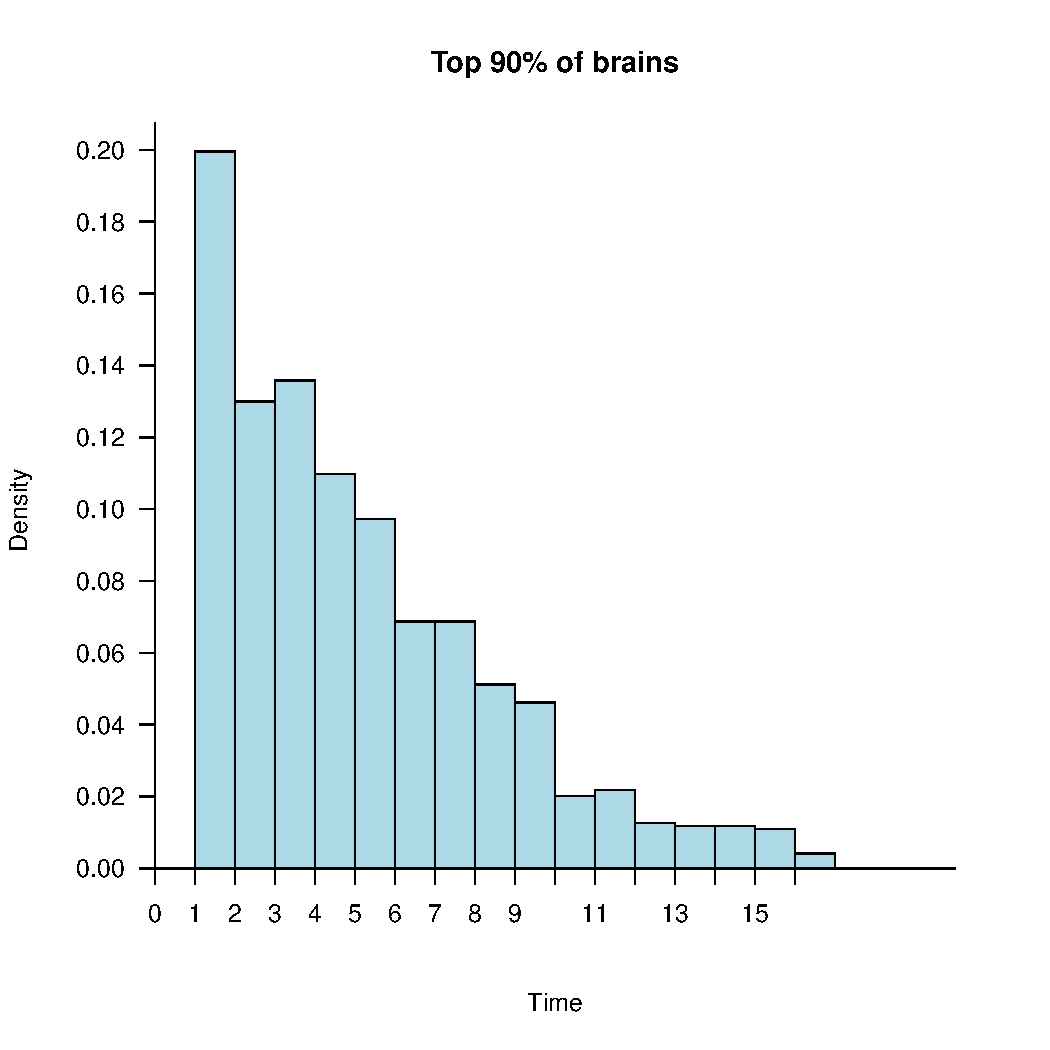
\includegraphics[width=100mm]{./Top90Brains.pdf}
	\caption{Top 90\% of Brains}
	\label{fig: 90_perc_brains_dist}
\end{figure}

\section{Conclusions}
Doing a partial state search is very expresive because each time a cell is filled in constraints have to be checked.

Conclusion
	Checking that cells satifies constraints is a very expensive operation And constraints have to be check every time a numeber is added.
	
	The perfomance is constrainted by hardware and Python language as it is an interpreted language.
	Take away message:
		There are many ways to solve a Sudoku puzzles using search methods. 
	Future work:
		Finding other ways to check constraints without 
		searchNxN:
			Finding a more effient way to select a square in the puzzle.
			Add an arc consistency to the puzzle.
		Brains:
			Choosing a better path to avoid recalculating the list of best nodes.


\end{document}
